
% Chapter Template
\setstretch{1}
\chapter{Prototype Development for Display Hardware}\thispagestyle{empty} % Main chapter title

\label{Chapter4} 

\lhead{Chapter 4. \emph{Prototype Development for Display Hardware}}
\setstretch{2}
\begin{figure}[!ht]
 \centering
  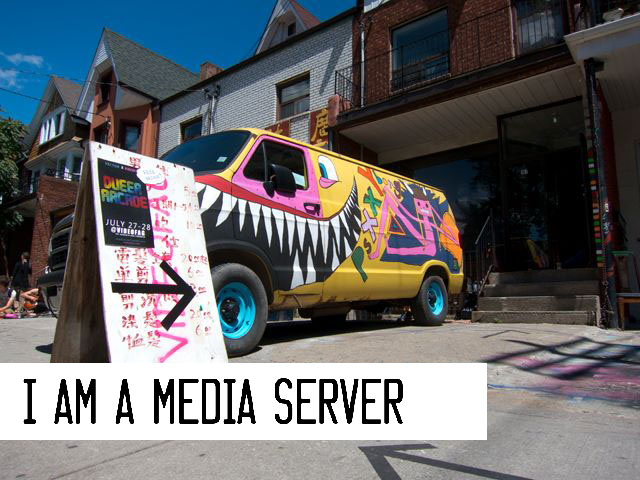
\includegraphics[width=\textwidth]{psXXYborgVan3}
  \caption{Hannah Epstein\\ psXXYborg at VideoFag, 1995}
\end{figure}

\clearpage
\begin{figure}[!ht]
 \centering
  \includegraphics[width=\textwidth]{ServerClientModel}
  \caption{screenPerfect interaction model between client, server, and studio.}
\end{figure}
\clearpage
\section{Client Server Model}

The chart in Figure 4.2 describes how screenPerfect's hardware serves a connection to a local cell phone, while occasionally obtaining software updates from the internet or from a direct upload when the resources are available for that upload. This is a useful model for public exhibition, because it does not require the device to be always-online with access to remote system resources. Instead, the software to run the artwork is stored locally and serves as both its own webserver and its own wifi hotspot, so that users can pair with the device on their own cell phone and interact with the art in public.

\section{Public Installations}
During the course of this project, games made with screenPerfect had many public outings. We installed \textit{psXXYborg} in a variety of spaces. There were a number of design approaches to the construction of those spaces. Hannah Epstein created many variations on space design, in including a straight projection on mylar, a whole-room space that would encompass the user in different projected, linked screens, and ultimately a portable "confessional" booth. The first variant of this is displayed in Figure 4.1, a custom-painted cargo van which we displayed at Videofag in Kensington Market as part of the Queer Arcade with Vector Art|Game Festival as part of their 2013 show (\url{http://www.vectorfestival.org/}).

More recent exhibitions of \textit{psXXYborg} have been built into a tent, which can be more easily displayed indoors. The \textit{psXXYborg} tent has been exhibited at Long Winter in December 2013 and at the Feminist Art Collective's annual conference at OCADu in 2014 (Figure 4.3). This helped to test and refine the list of design constraints for a successful work.

\clearpage
\begin{figure}[!ht]
 \centering
  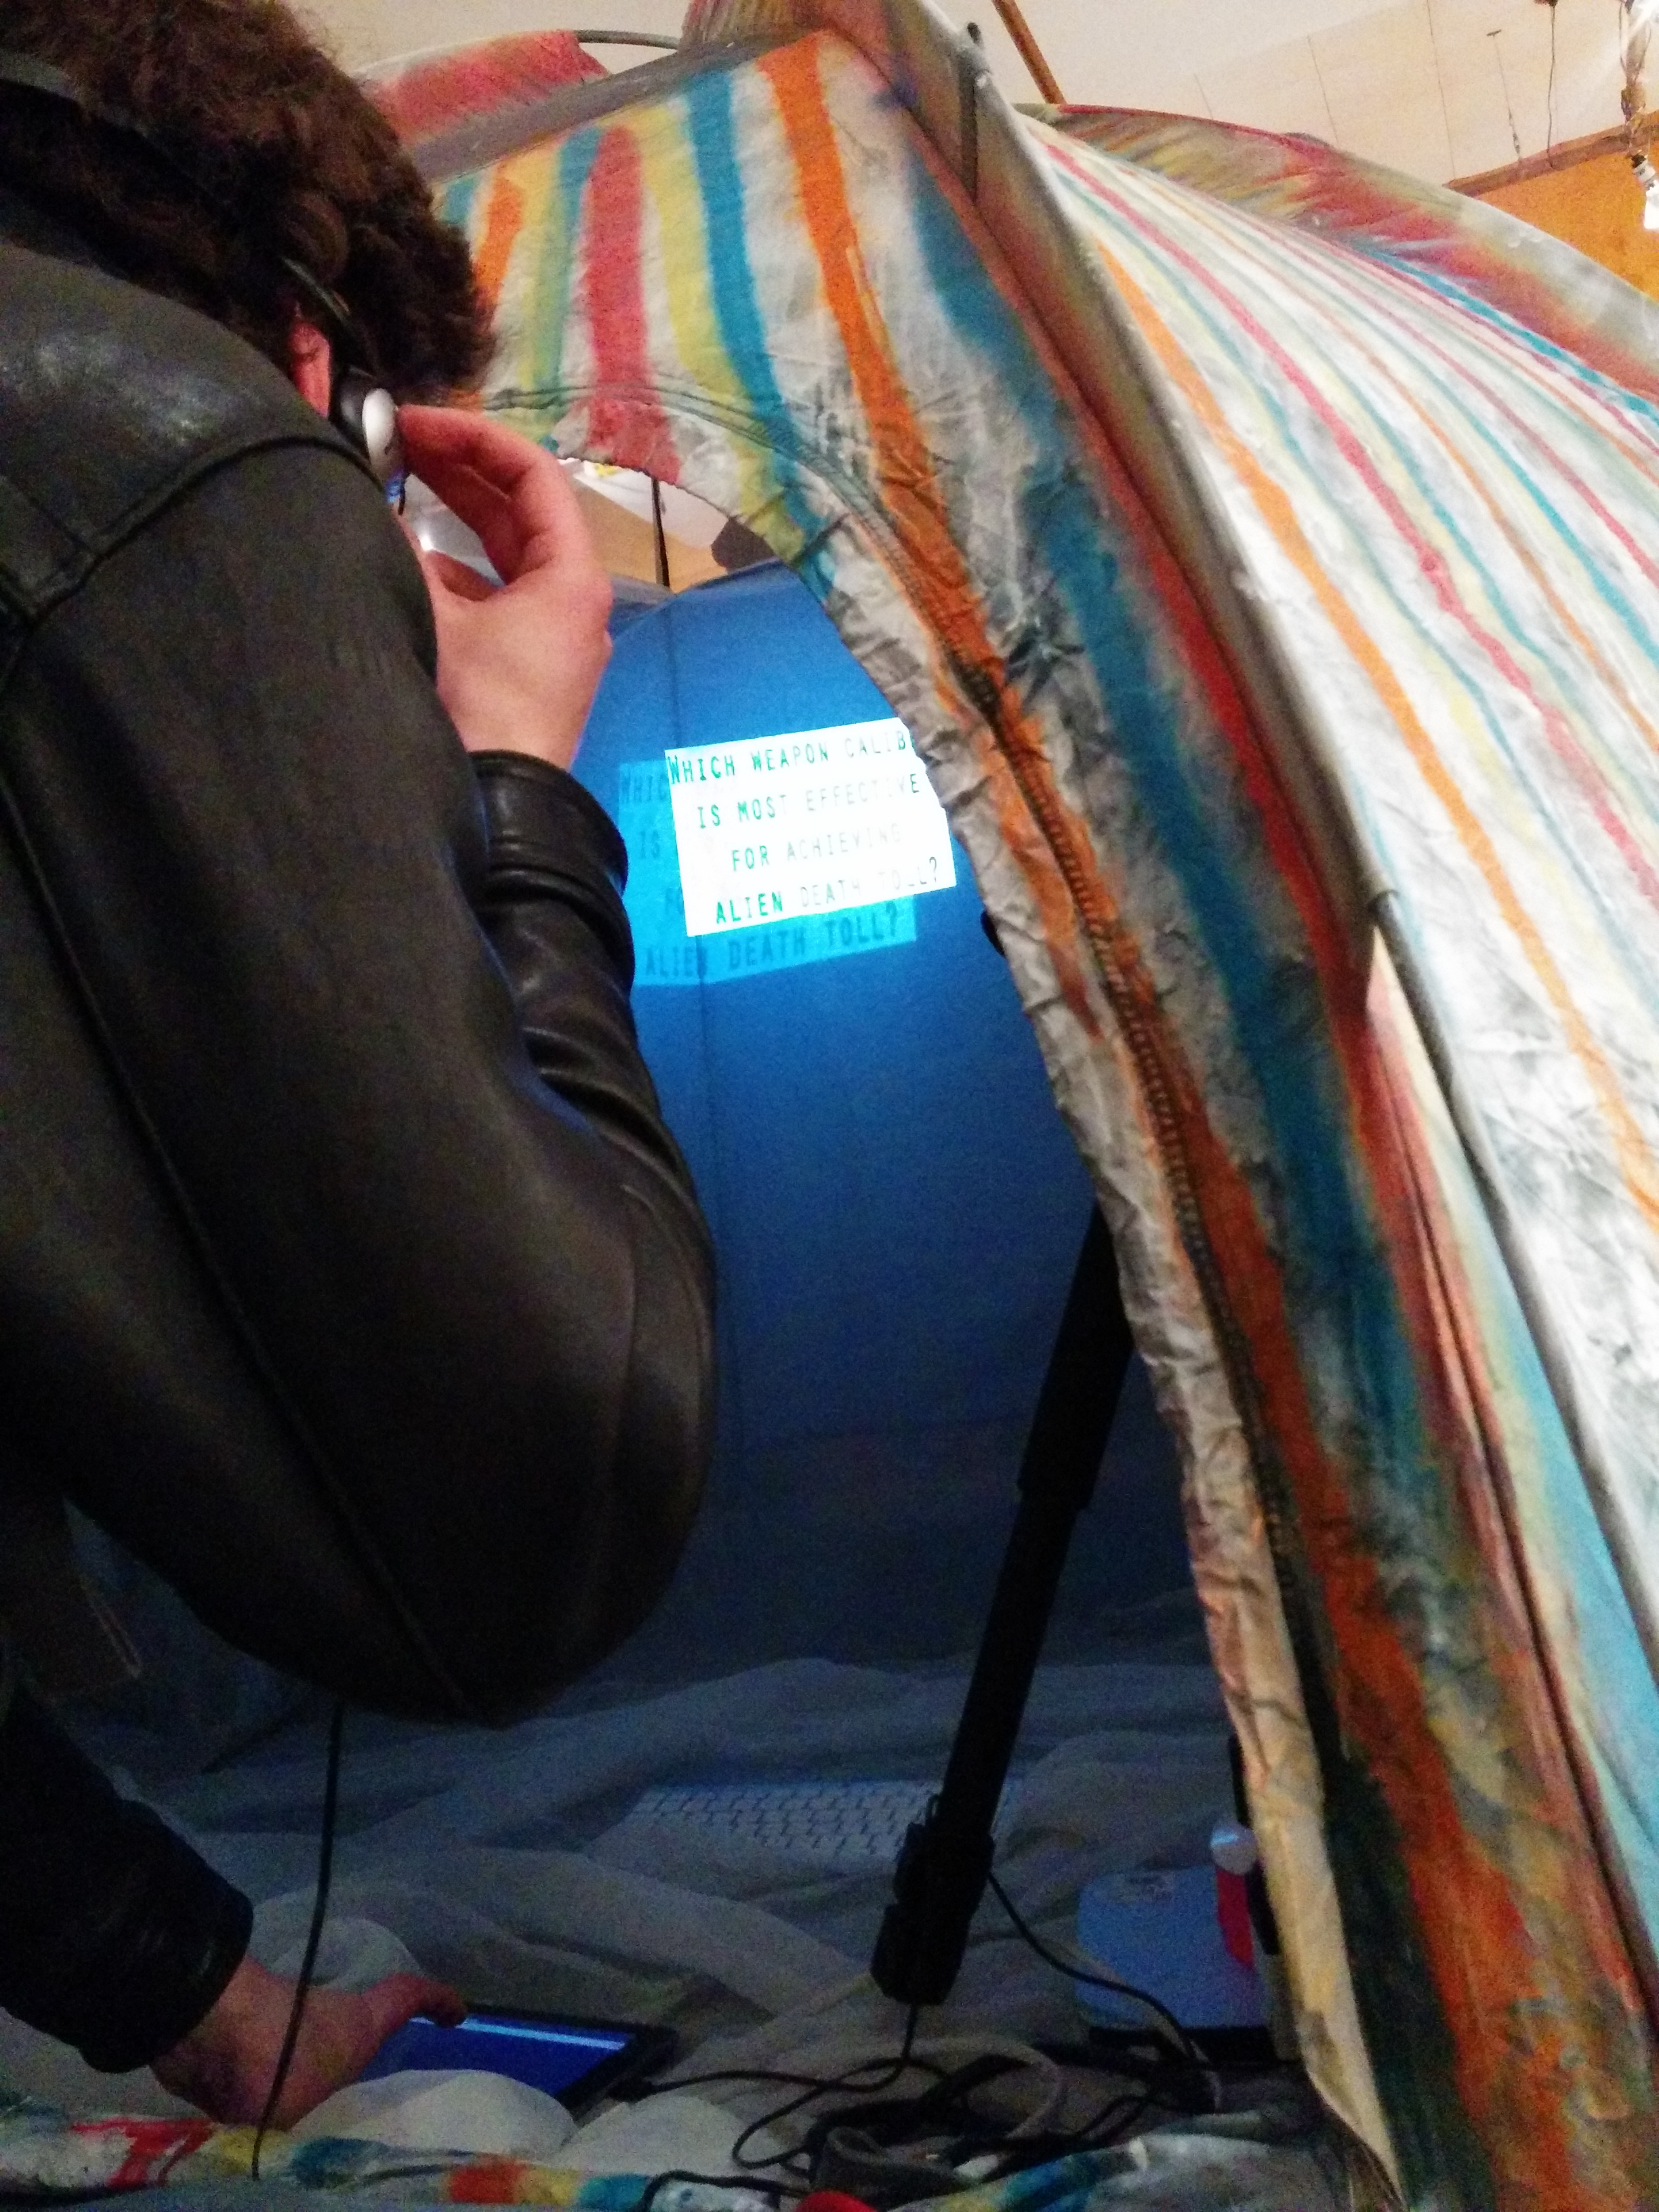
\includegraphics[width=0.7\textwidth]{psXXYborgTentPlay}
  \caption{Hannah Epstein\\\textit{psXXYborg} at FAC 2014, playthrough view}
\end{figure}
\clearpage

\section{Hardware Design}
The success of a project like screenPerfect is dependent not only on its software, or on its ease of use, but on how easy it is to install on-site. The software is dependent on open wifi and high bandwidth to communicate with client devices, a stable computing system, and a variety of computer interfaces. Ideally, the software is open and will work according to standards published by the W3C. In reality, it is incredibly difficult to build a new software system to work on broad platforms.

The following is a list of complications and assumptions built into the design of this hardware, based on public display experiences: 

\begin{enumerate}
\item Data service to an external source cannot be assumed to be available. 
\item The exhibit is assumed to be displayed in public.
\item The environment is assumed to be meterologically hostile - hot or cold, wet or very dry, and to be hosting at least one party, such as an art opening.
\item The exhibition is assumed to be supervised by technically untrained people.
\item The emphasis of the work should be on the work's display, rather than on a laptop screen.
\item The collectors of the work are assumed to have extremely limited resources for rugged workstations.
\item Any host-provided data carriage for external connection - wifi - is assumed to be overloaded by default.
\end{enumerate}

These are all very real constraints that impact display of interactive digital art. We use computers for work and play, but we still separate our lives into periods when we pursue one or the other. There are still boundaries between our personal and public lives. To use the same machines to display art as we do to build the work is to reduce the work from something approachable and consciously displayed to any other tab in a computer. It is my view that digital works especially must be seen within their exhibition context to be understood.

Because the display system needs to be stable and specfic but does not need to be used for development, I began to look into appliance-appropriate hardware. There are a number of low-power ARM-controller based hardware platforms on the market at the time of writing, including the Arduino, the Beagle Bone, and the Raspberry Pi. All of these systems are designed to help artists make interactive works that take advantage of computing power for expression. The Arduino is a popular system for learning to build electronic interactions, the Beagle Bone a full-featured Linux computer, and the Raspberry Pi has come out of an idealistic foundation that hopes to encourage people to learn to program and work with ultra-simplified computing systems.

The Raspberry Pi is my choice for building a hardware installation system to support screenPerfect. The Pi plugs directly into a television set for a monitor, uses Debian Linux for package control, and can store its entire operating system and dependent software on an SD Card - easy to image. Package control means that when one installs software on Debian, the software tends to maintain its own dependencies, which reduces the amount of time a programmer spends adding and removing libraries to get something simple to work. Where an Arduino would require an entire secondary shield to access the internet, the Raspberry Pi is a full computer out of the box, able to access the internet while still being useful from the command line. In addition to this, the computer is the size of a credit card, which makes it straightforward to install in an artistic location such as a van or tent. 

The Raspberry Pi as a platform is also affordable, at \$35 for a Model B with ethernet port and 512Mb of RAM. The Raspberry Pi foundation is a not-for-profit formed to support the opening of technical education to a broad range of children in the UK and overseas. This fit with the ideological stance of game::play Lab and the DMG, as well as my personal politics: that people should be able to use their tools as they see fit. Technology should serve its users, rather than requiring the user to serve technology.

\section{Technical Display Concerns and the Public Private Internet}
screenPerfect's technical display challenges have been embedded in limited systems, such as a reliance on institutional wireless, designed to block filesharing, which also block peer-to-peer experiments such as screenPerfect's server from connecting to its client computers. This resulted in a need for a portable wireless hotspot to serve the application reliably, as in addition to blocking institutional routers, too many users would overwhelm the service. This provided a direction for my primary development to take: the project needed a computer that served both its own web application and provided its own infrastructure, from being turned on to when it was turned off, which did not require any kind of specialized setup for display. In addition, I began to consider how screenPerfect might exist in public space without the requirement of a "smart" screen or any kind of specialized interaction equipment.

People are willing to use their smartphones publicly, but mainly to access the external internet, or messaging services while they are on the move. This led me to consider how people interact with the internet publicly and to consider topics of privacy and public space within the context of how these problems have already been solved by galleries and coffee shops wishing to offer their clientele data services to promote engagement.

In public spaces, internet is supplied by wifi, which comes through a specific type of router known as a "captive portal." A user will walk into a shop, attach to a network, and "sign" an agreement to make use of the wifi within that space. 

Normally, wifi will then give them access to the external internet - the internet as supplied by a major ISP. 
The Raspberry Pi installation of screenPerfect is instead a captive portal, which simultaneously supplies a wifi hotspot and a server that supplies information to that hotspot, without providing external access to the broader internet. This is similar to the pioneering 2013 Eyebeam project \textit{Subnod.es}, in which users pair to a captive portal which is also a server, supplying access to an entirely private chat room, which is available only to users on the network supplied by its own captive portal. 

The first issue addressed by this approach is that there is an inherent contradiction between downloading a site-specific piece to a personal device when the installed context is a core component of the aesthetic experience. Downloading applications to a smartphone seems invasive, particularly if those applications are experimental or site-specific, as I think that screenPerfect games are when they are at their best. The next is that web applications are very much not user-specific - they can be experienced anywhere while they are on the open web, even if their content is intended to be restricted to a specific type of installation, or requires it for best use. By serving the application locally, there is no reliance on an outside pipe. A copy of the game can be sold, customised, and stored in a collection, if such is desired, or installed in any kind of specific cabinet for later use.

\subsection{Subnod.es and Public Private Space}
This project has a precursor using similar technology built at Eyebeam in New York in 2013. Subnod.es uses a captive portal to display a chat client to only the local environment. The differences between screenPerfect and subnod.es are substantial, although mainly located within the code. Subnod.es relies on an external DNS being made available via the actual subnod.es software and depends on a different collection of software to serve the portal proper. It is also built such that those library dependencies are inseparable from the main project script.

The chief concern of subnod.es is that it was built as a response to concerns about communications privacy in North America under the NSA. Specifically, the author of subnod.es is concerned that people behave differently when they are watched, a subset of the concerns generally associated with panoptica and totalitarianism. While I have not specifically structured screenPerfect's Art Portal to address these concerns, it has been built to be largely private. It serves an application to a limited selection of a public space.

The assumption of screenPerfect is that galleries have limited resources but that people who go to art galleries almost certainly have access to a smart phone, which is a form of private space. Smart phones are people's own homes and are built to assume that they will stay with their owners at all times. This means that to install an app is to ask a lot of a viewer: specifically, it is to ask someone to bring an application into their private space without getting to sample it first. In contrast, serving that same application on the broad internet is to entirely delimit the context the art may be experienced within, which reduces its scarcity value to almost nothing while simultaneously removing the curator's ability to set the context of an exhibition experience. This means that it is unlikely an artist can be compensated in any conventional sense despite their large audience. It also means that the curation of the exhibit is no different than the "curation" found on Tumblr.

A better outcome might be to make a limited public space available in a private context. This is what we are doing when we ask that people open their phones and look at a website. The internet is the new public space. By presenting a web application using public technology within the exclusive context of the gallery - or desert, or forest - we take control again over how our art is presented. A gallery or exhibit space can be set up very specifically for the benefit of an audience in a way that the internet in general cannot be. Web technologies are a good solution for this because they are uniform and open in the way that more custom projection design software is not.

This sense of limited private space is key to the code-switching that human communication relies on. We are not the same people in public as we are in private. We are again different people when we are in different publics, from work to the street to school to the gallery. Technology that sensitively addresses these different code contexts seems likely to benefit its authors and users both by permitting the integration of the personal focus with a personal device with the context of a semi-public facility or "safe space" for engagement with the art work.

Safe space is space that has been constructed with an inclusivity policy to promote exploration and community-building within minority groups. It is intended as a systemic resistance to implicit violence. 

\section{Distribution of Work}
An optimal route to distribute both screenPerfect and the works produced with the tool is to compile them on an SD Card using the node-webkit package, which permits the distribution of web applications as desktop software without losing the multi-device communication channels supplied by a webserver. This could then be distributed digitally over the internet.

Futher, screenPerfect has already been forked. The system is publicly available on Github to permit anyone to extend the software. The Node.JS package can be compiled to include Windows, Linux, and OSX distributions, as well as being installed directly to a Raspbian - Raspberry Pi Debian - operating system, which would then launch the game or tools on boot. 

